\section{INTERCEPT TIMELINES}

\subsection{TERMINOLOGY}

\begin{tcoloritemize}
    \blueitem[Contact]
    \blueitem[Group]
    \blueitem[Picture]
\end{tcoloritemize}

\subsection[AR FLOW]{ACTIVE-RADAR MISSILE FLOW}

\begin{tcoloritemize}
    \blueitem[Launch-and-Leave]
    Launch-and-leave tactics utilize AIM-120 terminal guidance independence 
    to defeat bandit missiles though out maneuvers, 
    with the fighter turning cold once AIM-120 has gone active.

    \bigskip
    \textbf{Skate} \hfill see \cref{subsec:ttpaa:timeline:skate}\\
    AIM-120 launched before a briefed tranisition range 
    such that it goes active before fighters reach a desired out range.
    Fighters go out before recommitting for a second launch.
    
    \bigskip
    \textbf{Short-Skate} \hfill see \cref{subsec:ttpaa:timeline:shortskate}\\
    AIM-120 launched such that fighter can go out before reaching MAR.

    \blueitem[Launch-and-Decide]
    Launch-and-decide tactics also utilize AIM-120 terminal guidance independence, 
    allowing fighter to decide whether to abort out or continue in.

    \bigskip
    \textbf{Banzai} \hfill see \cref{subsec:ttpaa:timeline:banzai}\\
    Fighter launches before a briefed decision range and goes into notch for predetermined duration. 
    Can abort out or continue in depending on if spiked/naked and bandit maneuver.

    Typically employed with elements cranking in opposite directions, increasing chance of 1 fighter being naked
\end{tcoloritemize}


\subsection{RANGE DEFINITIONS}

\begin{tcoloritemize}
    \blueitem[Bandit WEZ] \textbf{W}eapon \textbf{E}ngagement \textbf{Zone}

    \medskip
    range at which bandit weapons can engage fighter, synonomous with bandit R\textsubscript{F-pole} in this document

    \blueitem[MAR] \textbf{M}inimum \textbf{A}bort \textbf{R}ange

    \medskip
    minimum range at which fighter can perform an abort maneuver to kinematically defeat any launched bandit weapons 

    \medskip
    \textbf{MAR} = max bandit R\textsubscript{F-pole} + fighter turn radius
    \blueitem[MSR] \textbf{M}inimum \textbf{S}hot \textbf{R}ange

    \medskip
    minimum range at which AIM-120 will go active before fighter reaches MAR if launched

    \blueitem[DOR] \textbf{D}esired \textbf{O}ut \textbf{R}ange

    \medskip
    minimum range at which fighter can go out, defeating bandit missiles, 
    before recommitting to a second employment with launch-and-decide tactics

    \blueitem[TR] \textbf{T}ransition \textbf{R}ange

    \medskip
    minimum range at which AIM-120 will go active before fighter reaches DOR if launched
    \blueitem[MTR] \textbf{M}inimum \textbf{T}argeting \textbf{R}ange

    \medskip
    minimum range for flight to begin targeting and execute launch-and-leave tactics
    \blueitem[MRR] \textbf{M}inimum \textbf{R}ecommit \textbf{R}ange

    \medskip
    minimum range at which a fighter which is out can recommit, 
    retarget and employ an AIM-120 before going out again at MAR

    \blueitem[DR] \textbf{D}ecision \textbf{R}ange

    \medskip
    minimum range at which fighter can execute briefed notch maneuver for launch-and-decide tactics

    \medskip

    \textbf{DR} = max bandit R\textsubscript{F-pole} + bandit closure \times \ t\textsubscript{notch}
\end{tcoloritemize}

\notebox{
    \small\textbf{\Crefrange{fig:ttpaa:timeline:banzai}{fig:ttpaa:timeline:shortskate} are not to scale, any crank maneuvers are ommitted for compactness.}
}

\marginfigeometry

\subsection{BANZAI TIMELINE}
\label{subsec:ttpaa:timeline:banzai}

\begin{checklistenumerate}[start=0]
    \blueitem[Pre-commit] maintain SA
    
    \begin{itemize}
        \item \textbf{Comms} --- monitor AWACS
        \item \textbf{Sensors} --- sanitize airspace
    \end{itemize}

    \blueitem[Commit]%
    \label{subsec:ttpaa:timeline:banzai:commit}
    \marginpar{
        \captionsetup{type=figure}
        \centering
        \begin{tikzpicture}[figstyle]

            % coordinates
            \coordinate (fighter_start) at (0,0);
            \coordinate (bandit) at (5,75);

            \coordinate (cr) at (0,0);
            \coordinate (mtr) at (0,10);
            \coordinate (sort) at (0,17.5);
            \coordinate (shoot) at (0,25);
            \coordinate (dr) at (0,35);
            \coordinate (fighter_banzai) at (20,55);
            \coordinate (fighter_abort) at (20,30);
            \coordinate (mar) at (5,50);
            \coordinate (wez) at (0,60);

            % range lines
            \draw[thin]
                (25,0) -- (25,75);

            \path let \p1=(bandit) in 
            node[font=\footnotesize,anchor=west] at (25,\y1) {BANDIT};
            \path let \p1=(wez) in 
            node[font=\footnotesize,anchor=west] at (25,\y1) {WEZ};
            \path let \p1=(mar) in 
            node[font=\footnotesize,anchor=west] at (25,\y1) {MAR};
            \path let \p1=(dr) in 
            node[font=\footnotesize,anchor=west] at (25,\y1) {DR};
            \path let \p1=(mtr) in 
            node[font=\footnotesize,anchor=west] at (25,\y1) {MTR};
            \path let \p1=(cr) in 
            node[font=\footnotesize,anchor=west] at (25,\y1) {CR};

            \draw[thin, dashed] let \p1=(wez) in  
                (25,\y1) -- ++(-30, 0);
            \draw[thin, dashed] let \p1=(mar) in  
                (25,\y1) -- ++(-30, 0);
            \draw[thin, dashed] let \p1=(dr) in  
                (25,\y1) -- ++(-25, 0);
            \draw[thin, dashed] let \p1=(mtr) in  
                (25,\y1) -- ++(-25, 0);
            \draw[thin, dashed] let \p1=(cr) in  
                (25,\y1) -- ++(-25, 0);

            % bandit wez
            \draw[fill=red!40]
                (bandit)
                -- ++(-60:15)
                arc (-60:-120:15)
                -- (bandit);
            
            % timeline
            \draw[->] 
                (fighter_start) -- 
                node[below, pos=0]{
                    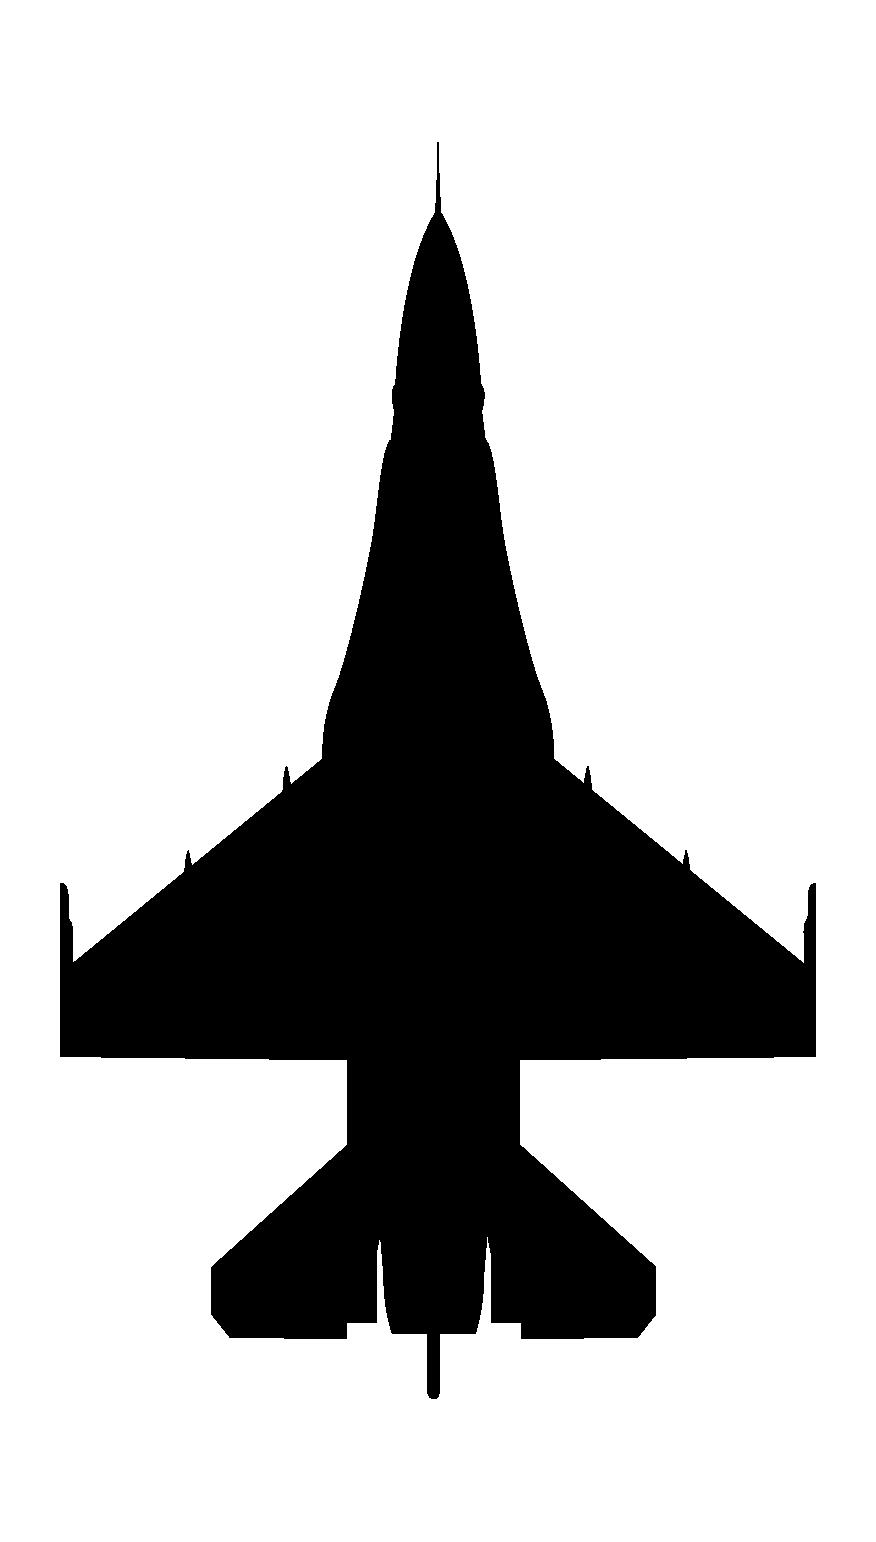
\includegraphics[
                    width=7.5mm,
                ]{diagrams/aircraft/silhouette_f16_top.pdf}} 
                (mtr);
            \draw[->]
                (mtr)
                -- (shoot);
            \draw[->]
                (shoot)
                -- (dr);
            \draw[->, dashed]
                (dr)
                arc (180:90:5) 
                -- ++(10,0)
                arc (90:0:5) 
                -- (fighter_abort)
                node[below, pos=1, ]{
                    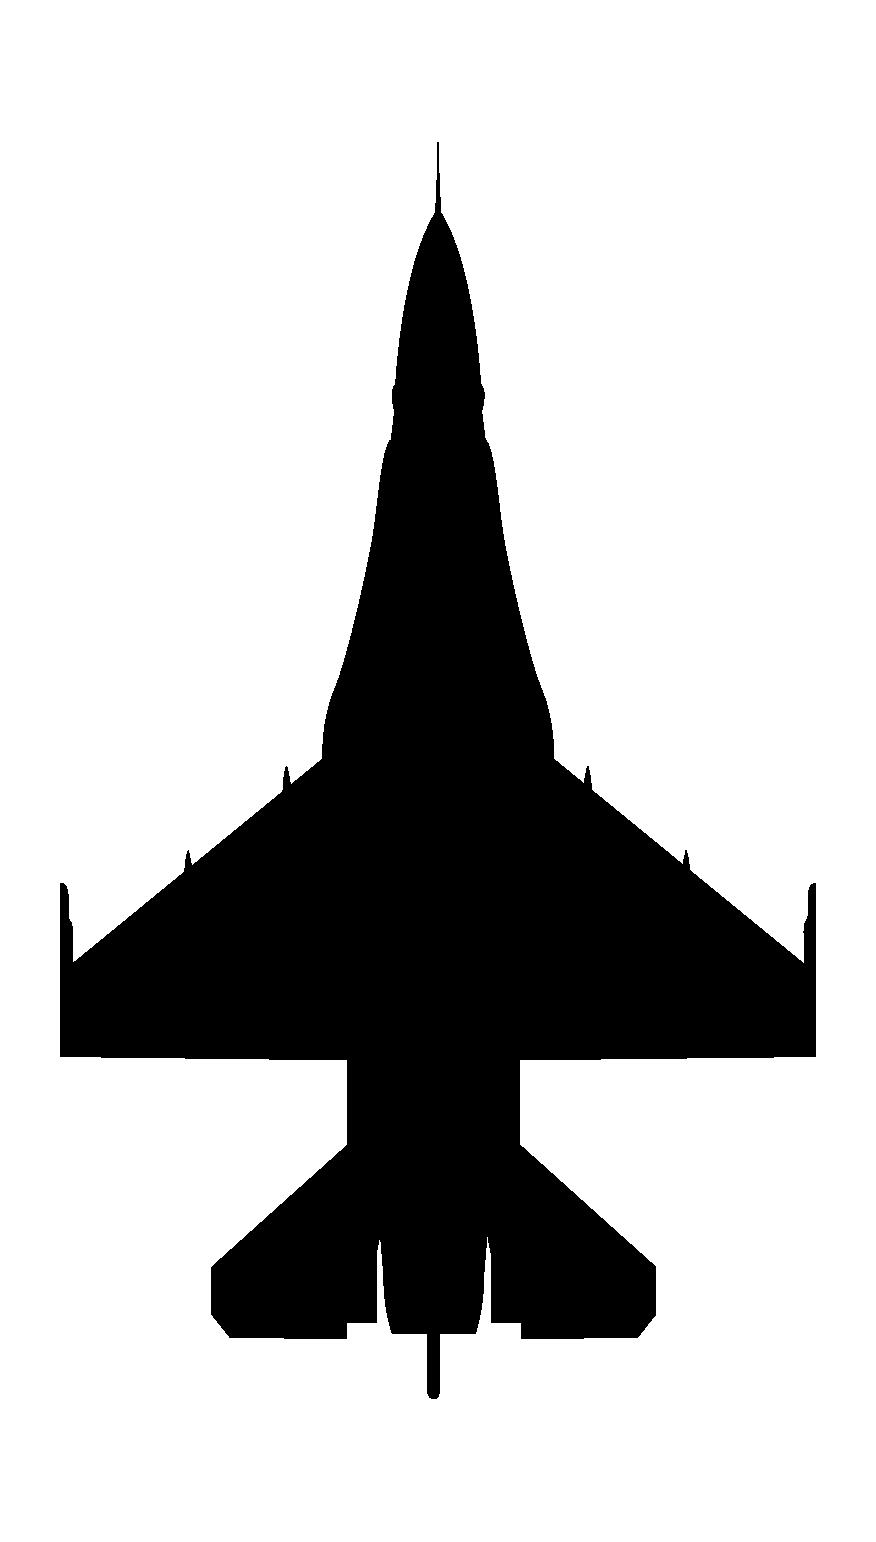
\includegraphics[
                        angle=180,
                        width=7.5mm,
                ]{diagrams/aircraft/silhouette_f16_top.pdf}};
            \draw[->]
                (dr)
                arc (180:90:5) 
                -- ++(10,0)
                arc (-90:0:5) 
                -- (fighter_banzai)
                node[above, pos=1, ]{
                    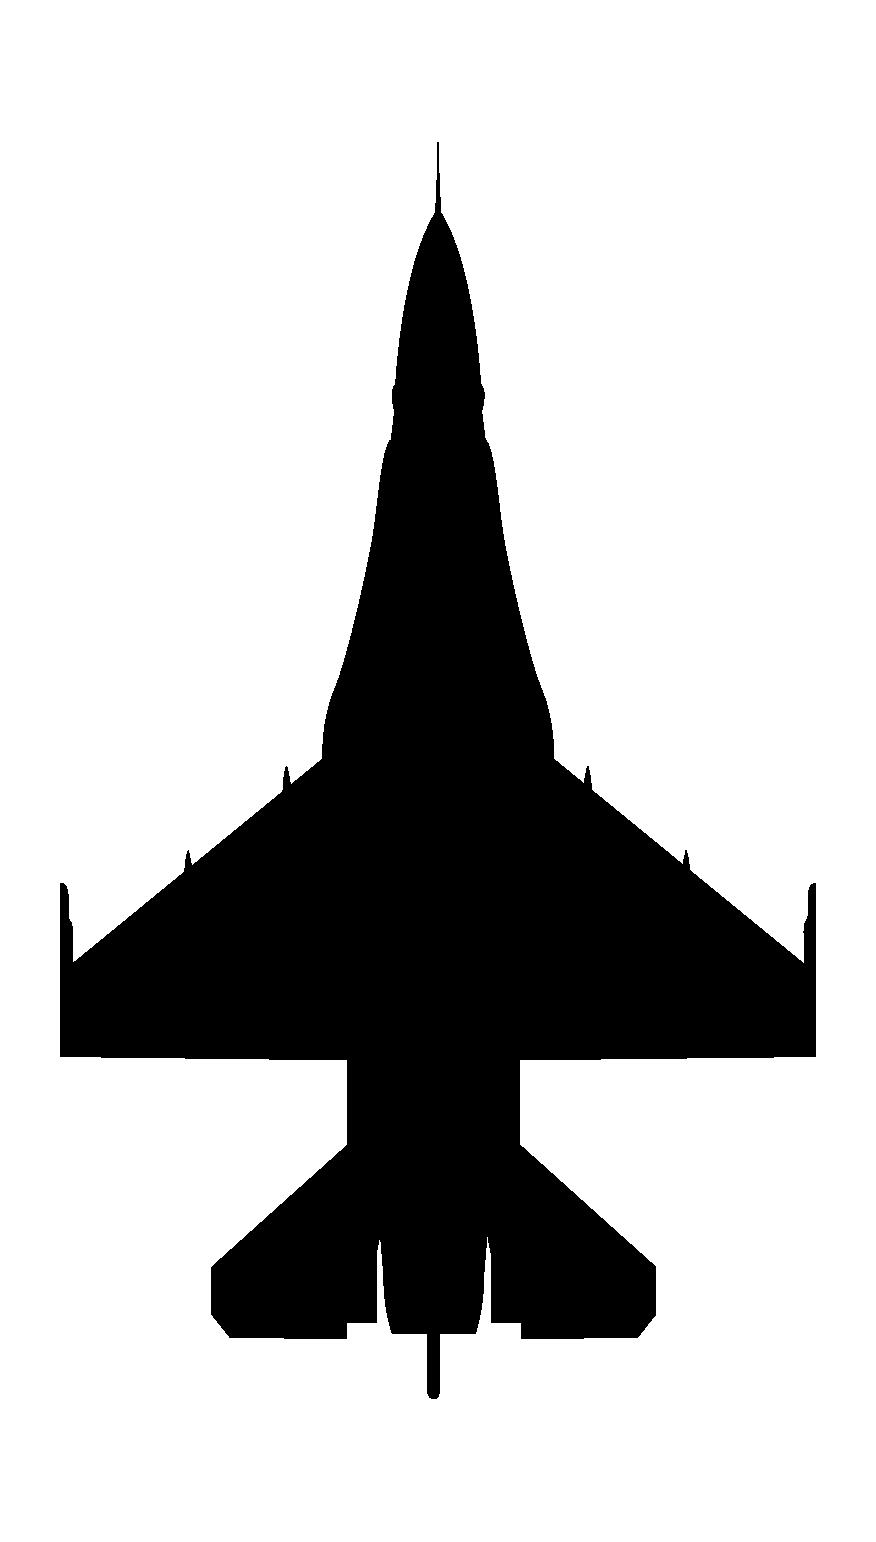
\includegraphics[
                        angle=0,
                        width=7.5mm,
                ]{diagrams/aircraft/silhouette_f16_top.pdf}};

            % bandit
            \node[] at (bandit) {
                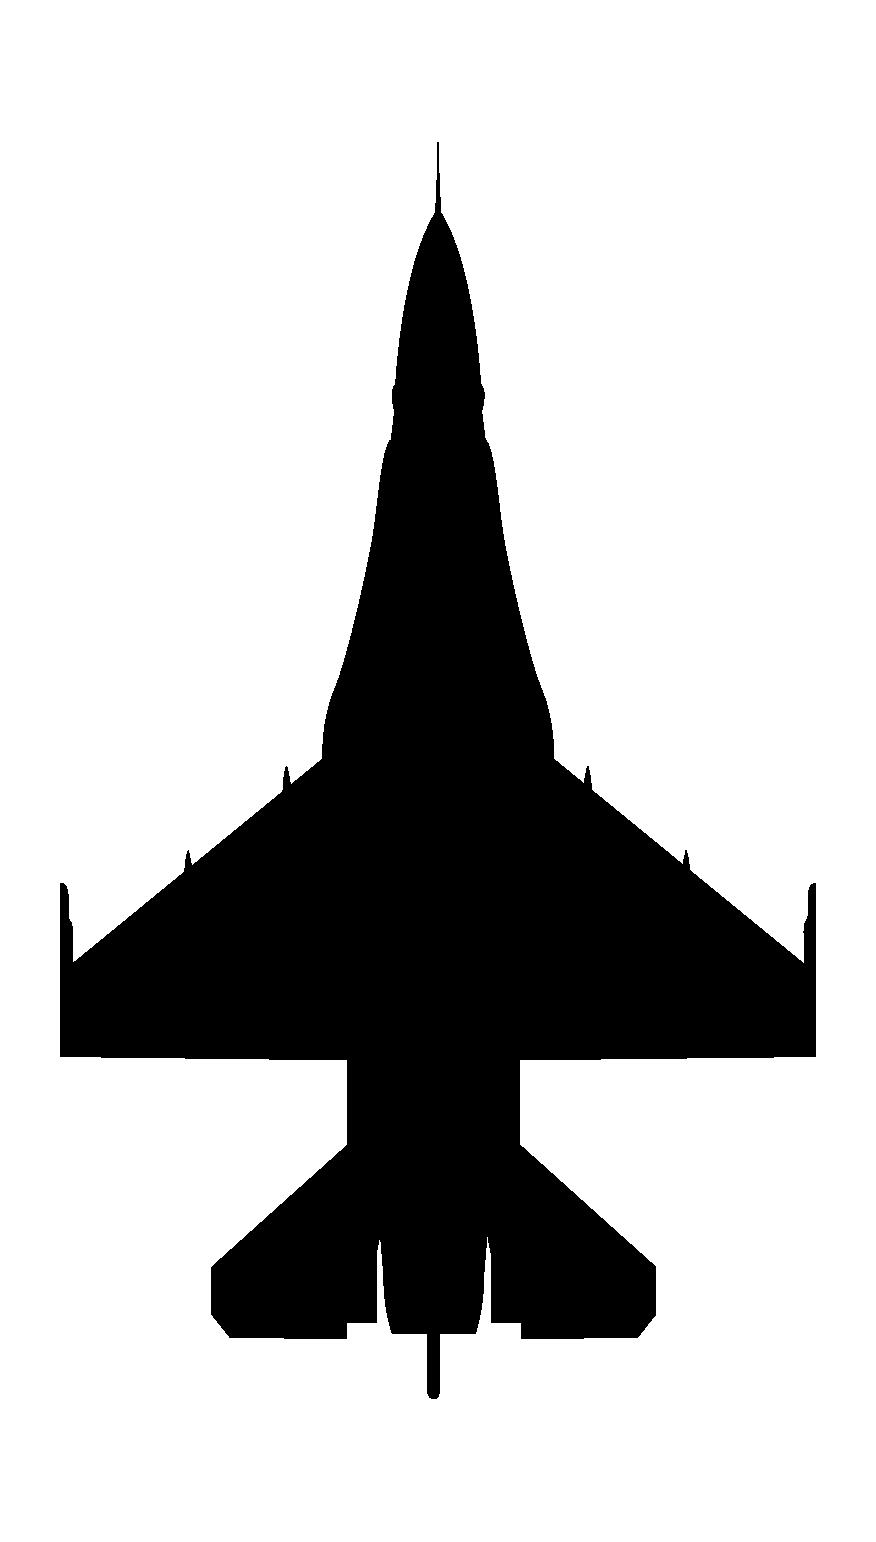
\includegraphics[
                    angle=180,
                    width=7.5mm,
            ]{diagrams/aircraft/silhouette_f16_top.pdf}};

            % labels
            \node[left, align=right, font=\small] at (cr) {
                \ref{subsec:ttpaa:timeline:banzai:commit}
            };
            \node[left, align=right, font=\small] at (mtr) {
                \ref{subsec:ttpaa:timeline:banzai:target}
            };
            \node[left, align=right, font=\small] at (sort) {
                \ref{subsec:ttpaa:timeline:banzai:sort}
            };
            \node[left, align=right, font=\small] at (shoot) {
                \ref{subsec:ttpaa:timeline:skate:shoot}
            };
            \node[left, align=right, font=\small] at (dr) {
                \ref{subsec:ttpaa:timeline:banzai:notch}
            };
            \node[left, align=right, font=\small] at (fighter_banzai) {
                \ref{subsec:ttpaa:timeline:banzai:banzai}
            };
            \node[left, align=right, font=\small] at (fighter_abort) {
                \ref{subsec:ttpaa:timeline:banzai:abort}
            };

        \end{tikzpicture}
        \caption{Banzai timeline}
        \label{fig:ttpaa:timeline:banzai}
    }%
    \textbf{--- start of intercept timeline}
    \begin{itemize}
        \item AWACS picture or own FCR contacts meet briefed commit criteria
        \item flight leaves assigned patrol area
        \item \textbf{No later than CR}
    \end{itemize}

    \blueitem[Target]
    \label{subsec:ttpaa:timeline:banzai:target}
    \begin{itemize}
        \item target call indicates responsibility to \\
        engage group in accordance with ROE
        \item flight members obtain radar contact
        \item \textbf{No later than MTR}
    \end{itemize}

    \blueitem[Sort]
    \label{subsec:ttpaa:timeline:banzai:sort}
    \begin{itemize}
        \item flight members sort contacts
        \item flight members obtain FCR lock on assigned contact
    \end{itemize}

    \blueitem[MRM Employment]
    \label{subsec:ttpaa:timeline:banzai:shoot}
    \begin{itemize} 
        \item verify clear avenue of fire
        \item \textbf{crank post launch to minimize closure}
        \item \textbf{such that missile active before fighter reaches DR}
    \end{itemize}
    
    \blueitem[Notch]
    \label{subsec:ttpaa:timeline:banzai:notch}
    \begin{itemize} 
        \item notch predetermined time (15s)
        \item \textbf{No later than DR}
    \end{itemize}
    \blueitem[Banzai / Abort]
    \begin{enumerate}[label=\textbf{\arabic{enumi}\alph*.}]
        \item \blue{Abort} (spiked) --- \textbf{5G slicing turn}%
        \label{subsec:ttpaa:timeline:banzai:abort}%
        \item \blue{Banzai} (naked) --- recommit and engage%
        \label{subsec:ttpaa:timeline:banzai:banzai}%
    \end{enumerate}
    
\end{checklistenumerate}

\clearpage

\subsection{SKATE TIMELINE}
\label{subsec:ttpaa:timeline:skate}

\begin{checklistenumerate}[start=0]
    \blueitem[Pre-commit] maintain SA
    
    \begin{itemize}
        \item \textbf{Comms} --- monitor AWACS
        \item \textbf{Sensors} --- sanitize airspace
    \end{itemize}

    \blueitem[Commit]%
    \label{subsec:ttpaa:timeline:skate:commit}
    \marginpar{
        \captionsetup{type=figure}
        \centering
        \begin{tikzpicture}[figstyle]

            % coordinates
            \coordinate (fighter_start) at (0,0);
            \coordinate (bandit) at (5,80);

            \coordinate (cr) at (0,0);
            \coordinate (mtr) at (0,10);
            \coordinate (sort) at (0,20);
            \coordinate (tr) at (0,30);
            \coordinate (dor) at (0,40);
            \coordinate (mrr) at (15,20);
            \coordinate (shoot2) at (5,50);
            \coordinate (mar) at (5,55);
            \coordinate (wez) at (0,65);
            \coordinate (fighter_end) at (20,50);

            % range lines
            \draw[thin]
                (25,0) -- (25,80);

            \path let \p1=(bandit) in 
            node[font=\footnotesize,anchor=west] at (25,\y1) {BANDIT};
            \path let \p1=(wez) in 
            node[font=\footnotesize,anchor=west] at (25,\y1) {WEZ};
            \path let \p1=(mar) in 
            node[font=\footnotesize,anchor=west] at (25,\y1) {MAR};
            \path let \p1=(dor) in 
            node[font=\footnotesize,anchor=west] at (25,\y1) {DOR};
            \path let \p1=(mrr) in 
            node[font=\footnotesize,anchor=west] at (25,\y1) {MRR};
            \path let \p1=(tr) in 
            node[font=\footnotesize,anchor=west] at (25,\y1) {TR};
            \path let \p1=(mtr) in 
            node[font=\footnotesize,anchor=west] at (25,\y1) {MTR};
            \path let \p1=(cr) in 
            node[font=\footnotesize,anchor=west] at (25,\y1) {CR};

            
            
            \draw[thin, dashed] let \p1=(wez) in  
                (25,\y1) -- ++(-30, 0);
            \draw[thin, dashed] let \p1=(mar) in  
                (25,\y1) -- ++(-20, 0);
            \draw[thin, dashed] let \p1=(dor) in  
                (25,\y1) -- ++(-25, 0);
            \draw[thin, dashed] let \p1=(tr) in  
                (25,\y1) -- ++(-25, 0);
            \draw[thin, dashed] let \p1=(mrr) in  
                (25,\y1) -- ++(-10, 0);
            \draw[thin, dashed] let \p1=(mtr) in  
                (25,\y1) -- ++(-25, 0);
            \draw[thin, dashed] let \p1=(cr) in  
                (25,\y1) -- ++(-25, 0);

            % bandit wez
            \draw[fill=red!40]
                (bandit)
                -- ++(-60:15)
                arc (-60:-120:15)
                -- (bandit);
            
            % timeline
            \draw[->] 
                (fighter_start) -- 
                node[below, pos=0]{
                    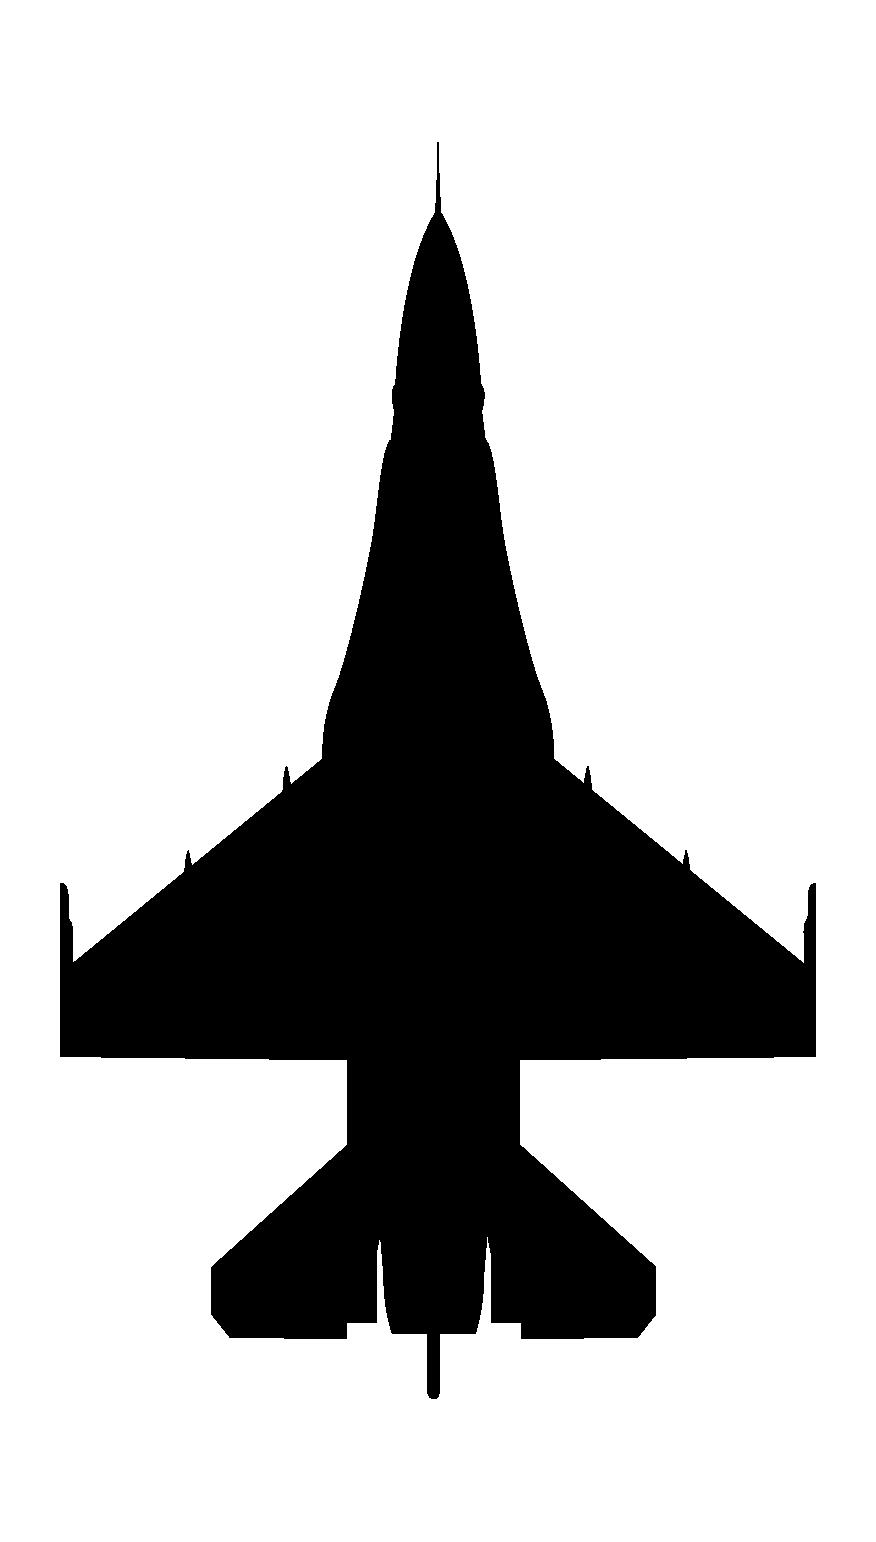
\includegraphics[
                    width=7.5mm,
                ]{diagrams/aircraft/silhouette_f16_top.pdf}} 
                (mtr);
            \draw[->]
                (mtr)
                -- (tr);
            \draw[->]
                (tr)
                -- (dor);
            \draw[->]
                (dor)
                arc (180:90:5) 
                -- ++(5,0)
                arc (90:0:5) 
                -- (mrr);
            \draw[->]
                (mrr)
                arc (0:-180:5) 
                -- (mar);
            \draw[->]
                (mar)
                arc (180:90:5) 
                -- ++(5,0)
                arc (90:0:5) 
                -- (fighter_end)
                node[below, pos=1, ]{
                    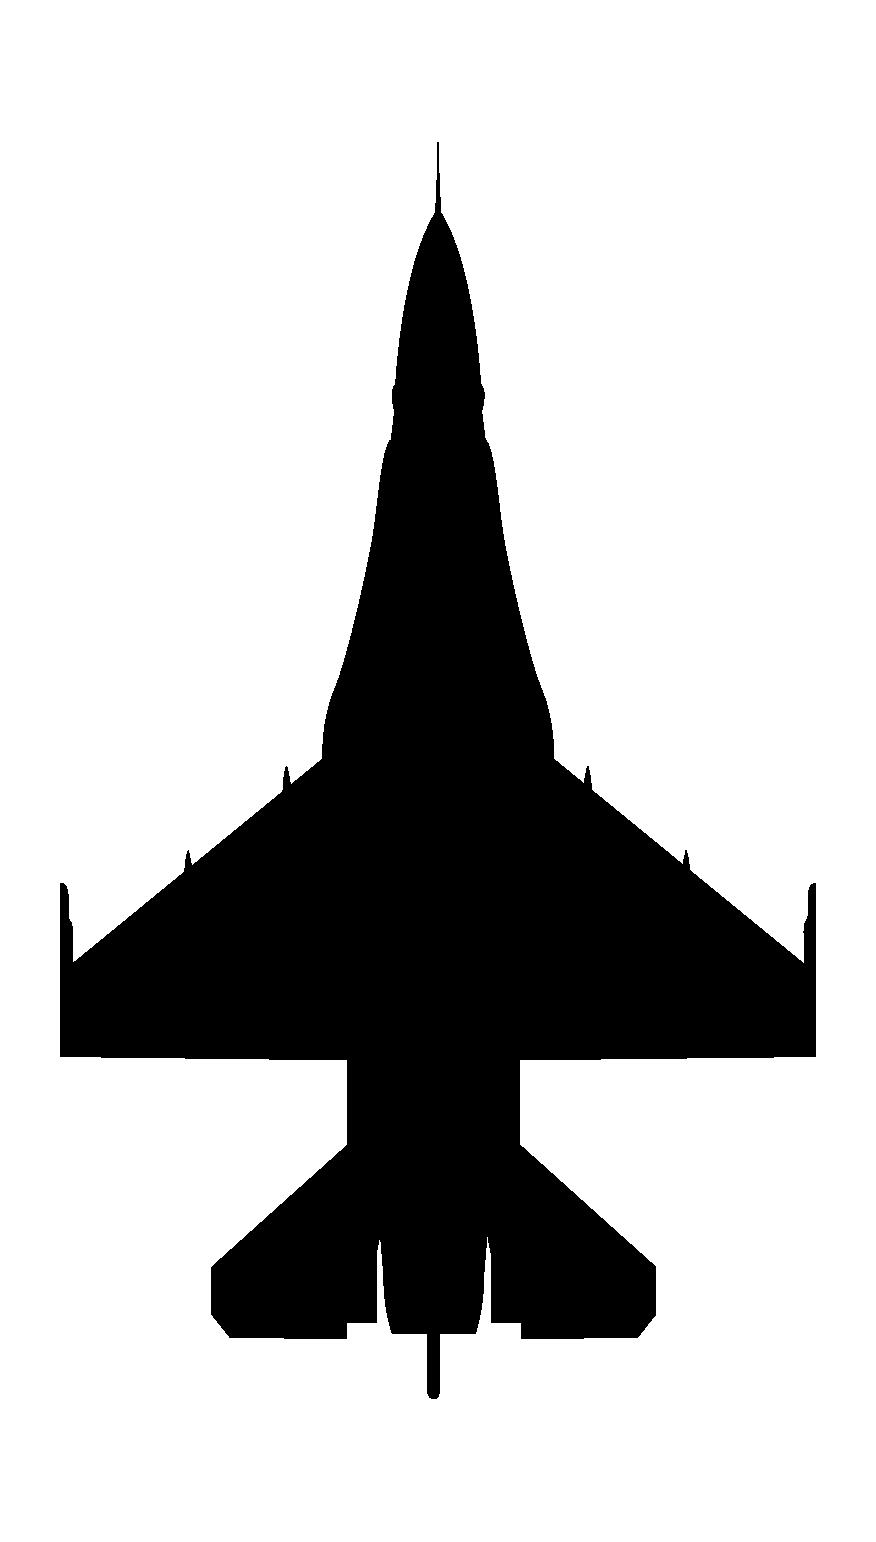
\includegraphics[
                        angle=180,
                        width=7.5mm,
                ]{diagrams/aircraft/silhouette_f16_top.pdf}};
            \draw[->, dashed]
                (mar)
                arc (180:90:5) 
                -- ++(5,0)
                arc (-90:0:5) 
                -- ++(0, 5)
                node[above, pos=1, ]{
                    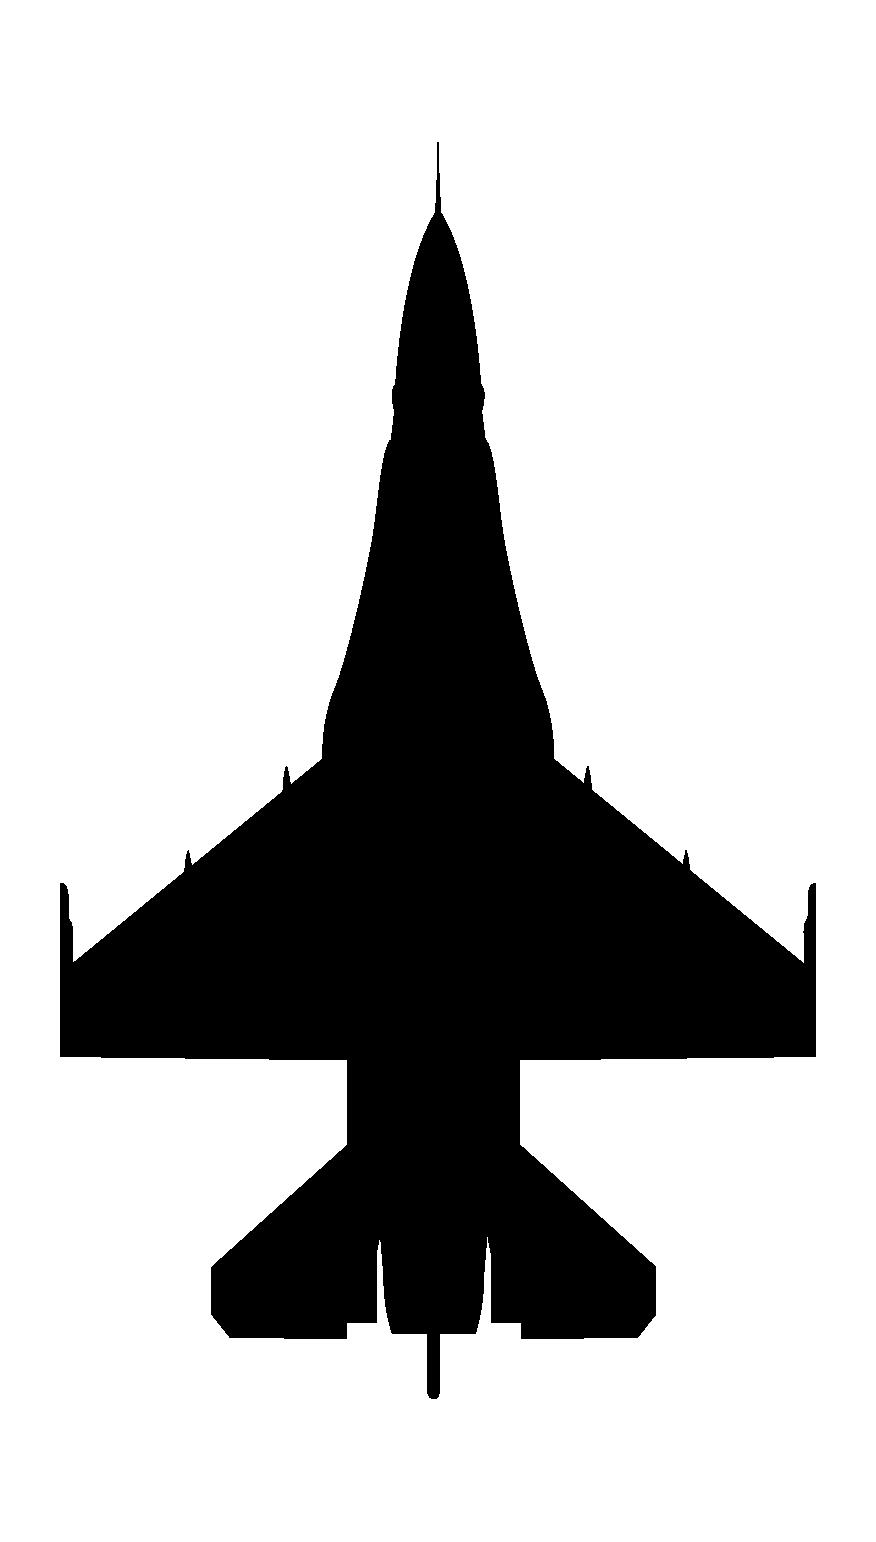
\includegraphics[
                        angle=0,
                        width=7.5mm,
                ]{diagrams/aircraft/silhouette_f16_top.pdf}};

            % bandit
            \node[] at (bandit) {
                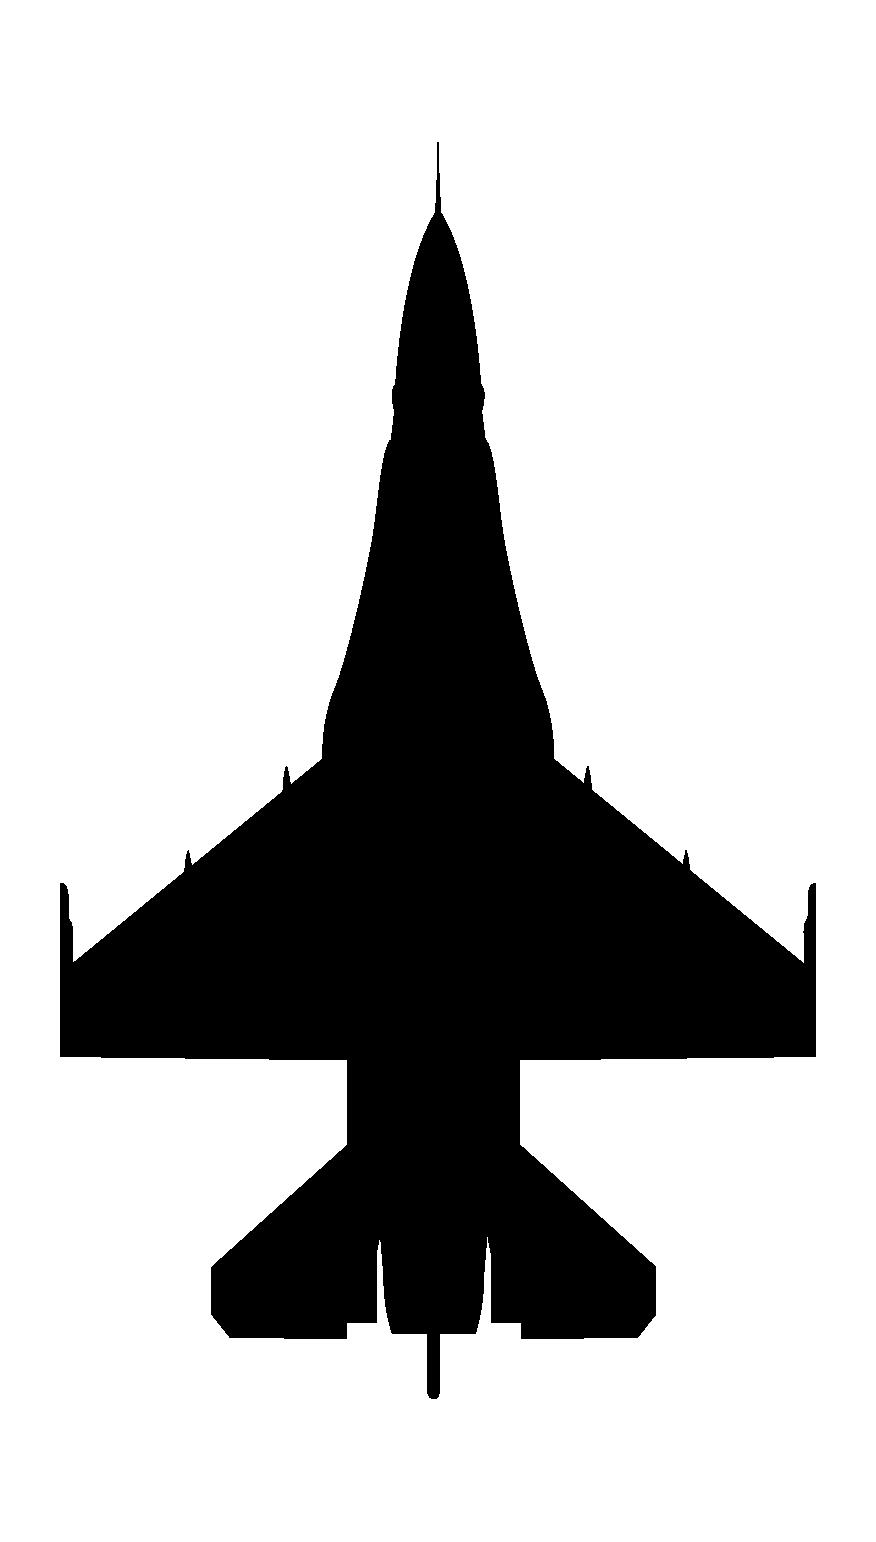
\includegraphics[
                    angle=180,
                    width=7.5mm,
            ]{diagrams/aircraft/silhouette_f16_top.pdf}};

            % labels
            \node[left, align=right, font=\small] at (cr) {
                \ref{subsec:ttpaa:timeline:skate:commit}
            };
            \node[left, align=right, font=\small] at (mtr) {
                \ref{subsec:ttpaa:timeline:skate:target}
            };
            \node[left, align=right, font=\small] at (sort) {
                \ref{subsec:ttpaa:timeline:skate:sort}
            };
            \node[left, align=right, font=\small] at (tr) {
                \ref{subsec:ttpaa:timeline:skate:shoot}
            };
            \node[left, align=right, font=\small] at (dor) {
                \ref{subsec:ttpaa:timeline:skate:out}
            };
            \node[left, align=right, font=\small] at (mrr) {
                \ref{subsec:ttpaa:timeline:skate:recommit}
            };
            \node[left, align=right, font=\small] at (shoot2) {
                \ref{subsec:ttpaa:timeline:skate:shoot2}
            };
            \node[left, align=right, font=\small] at (mar) {
                \ref{subsec:ttpaa:timeline:skate:abort}
            };

        \end{tikzpicture}
        \caption{Skate timeline}
        \label{fig:ttpaa:timeline:skate}
    }%
    \textbf{--- start of intercept timeline}
    \begin{itemize}
        \item AWACS picture or own FCR contacts meet briefed commit criteria
        \item flight leaves assigned patrol area
        \item \textbf{No later than CR}
    \end{itemize}

    \blueitem[Target]
    \label{subsec:ttpaa:timeline:skate:target}
    \begin{itemize}
        \item target call indicates responsibility to \\
        engage group in accordance with ROE
        \item flight members obtain radar contact
        \item \textbf{No later than MTR}
    \end{itemize}

    \blueitem[Sort]
    \label{subsec:ttpaa:timeline:skate:sort}
    \begin{itemize}
        \item flight members sort contacts
        \item flight members obtain FCR lock on assigned contact
    \end{itemize}

    \blueitem[MRM Employment]
    \label{subsec:ttpaa:timeline:skate:shoot}
    \begin{itemize} 
        \item verify clear avenue of fire
        \item \textbf{DLZ} --- R\textsubscript{PI} to R\textsubscript{OPT}
        \hfill (see \cref{fig:ttpaa:timeline:skate:dlz})\\
        manual loft to maximize performance
        \item \textbf{crank post launch to minimize closure}
        \item \textbf{No later than TR}
    \end{itemize}
    
    \marginpar{
        \captionsetup{type=figure}
        \centering
        \begin{tikzpicture}[figstyle]
            \node[boxedmarfigstyle] (fig) at (0,0) {
                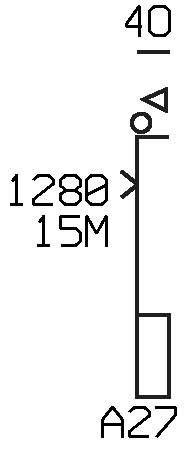
\includegraphics[
                    scale=0.5,
                ]{mfd/fcr_aa/aim120_subfig_dlz_prelaunch.pdf}
            };
        \end{tikzpicture}
        \caption{DLZ for skate}
        \label{fig:ttpaa:timeline:skate:dlz}
    }

    \blueitem[Out]
    \label{subsec:ttpaa:timeline:skate:out}
    \begin{itemize}
        \item \textbf{No later than DOR, after pitbull}
        \item 5G slicing turn
    \end{itemize}
    \blueitem[Recommit] (if necessary)
    \label{subsec:ttpaa:timeline:skate:recommit}
    \begin{itemize}
        \item \textbf{range must be greater than MRR}
        \item fighter must reacquire \& sort bandit
    \end{itemize}
    \blueitem[MRM Employment]
    \label{subsec:ttpaa:timeline:skate:shoot2}
    \begin{itemize}
        \item \textbf{No later than MAR}
    \end{itemize}
    \blueitem[Abort]%
    \label{subsec:ttpaa:timeline:skate:abort}
    \textbf{--- 5G slicing turn at MAR}
\end{checklistenumerate}

\clearpage

\subsection{SHORT SKATE TIMELINE}
\label{subsec:ttpaa:timeline:shortskate}

\begin{checklistenumerate}[start=0]
    \blueitem[Pre-commit] maintain SA
    
    \begin{itemize}
        \item \textbf{Comms} --- monitor AWACS
        \item \textbf{Sensors} --- sanitize airspace
    \end{itemize}

    \blueitem[Commit]%
    \label{subsec:ttpaa:timeline:shortskate:commit}
    \marginpar{
        \captionsetup{type=figure}
        \centering
        \begin{tikzpicture}[figstyle]

            % coordinates
            \coordinate (fighter_start) at (0,0);
            \coordinate (bandit) at (0,80);

            \coordinate (cr) at (0,0);
            \coordinate (mtr) at (0,10);
            \coordinate (sort) at (0,20);
            \coordinate (tr) at (0,30);
            \coordinate (msr) at (0,40);
            \coordinate (mar) at (0,55);
            \coordinate (wez) at (0,65);
            \coordinate (fighter_end) at (15,50);

            % range lines
            \draw[thin]
                (20,0) -- (20,80);

            \path let \p1=(bandit) in 
            node[font=\footnotesize,anchor=west] at (20,\y1) {BANDIT};
            \path let \p1=(wez) in 
            node[font=\footnotesize,anchor=west] at (20,\y1) {WEZ};
            \path let \p1=(mar) in 
            node[font=\footnotesize,anchor=west] at (20,\y1) {MAR};
            \path let \p1=(msr) in 
            node[font=\footnotesize,anchor=west] at (20,\y1) {MSR};
            \path let \p1=(tr) in 
            node[font=\footnotesize,anchor=west] at (20,\y1) {TR};
            \path let \p1=(mtr) in 
            node[font=\footnotesize,anchor=west] at (20,\y1) {MTR};
            \path let \p1=(cr) in 
            node[font=\footnotesize,anchor=west] at (20,\y1) {CR};

            
            
            \draw[thin, dashed] let \p1=(wez) in  
                (20,\y1) -- ++(-30, 0);
            \draw[thin, dashed] let \p1=(mar) in  
                (20,\y1) -- ++(-20, 0);
            \draw[thin, dashed] let \p1=(msr) in  
                (20,\y1) -- ++(-20, 0);
            \draw[thin, dashed] let \p1=(tr) in  
                (20,\y1) -- ++(-20, 0);
            \draw[thin, dashed] let \p1=(mtr) in  
                (20,\y1) -- ++(-20, 0);
            \draw[thin, dashed] let \p1=(cr) in  
                (20,\y1) -- ++(-20, 0);

            % bandit wez
            \draw[fill=red!40]
                (bandit)
                -- ++(-60:15)
                arc (-60:-120:15)
                -- (bandit);
            
            % timeline
            \draw[->] 
                (fighter_start) -- 
                node[below, pos=0]{
                    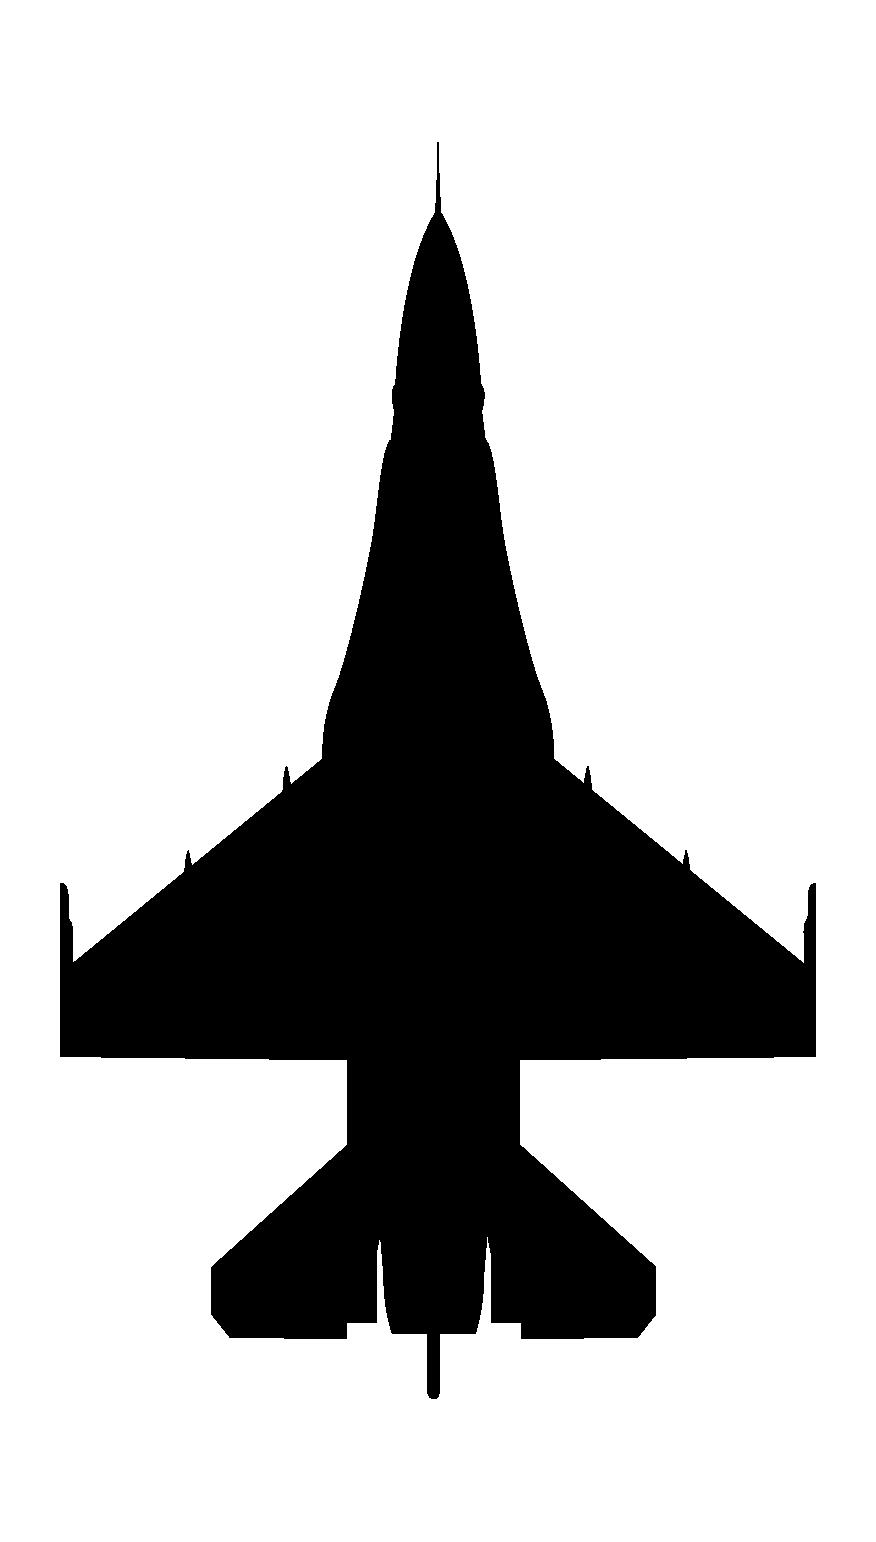
\includegraphics[
                    width=7.5mm,
                ]{diagrams/aircraft/silhouette_f16_top.pdf}} 
                (mtr);
            \draw[->]
                (mtr)
                -- (msr);
            \draw[->]
                (msr)
                -- (mar);
            \draw[->]
                (mar)
                arc (180:90:5) 
                -- ++(5,0)
                arc (90:0:5) 
                -- (fighter_end)
                node[below, pos=1, ]{
                    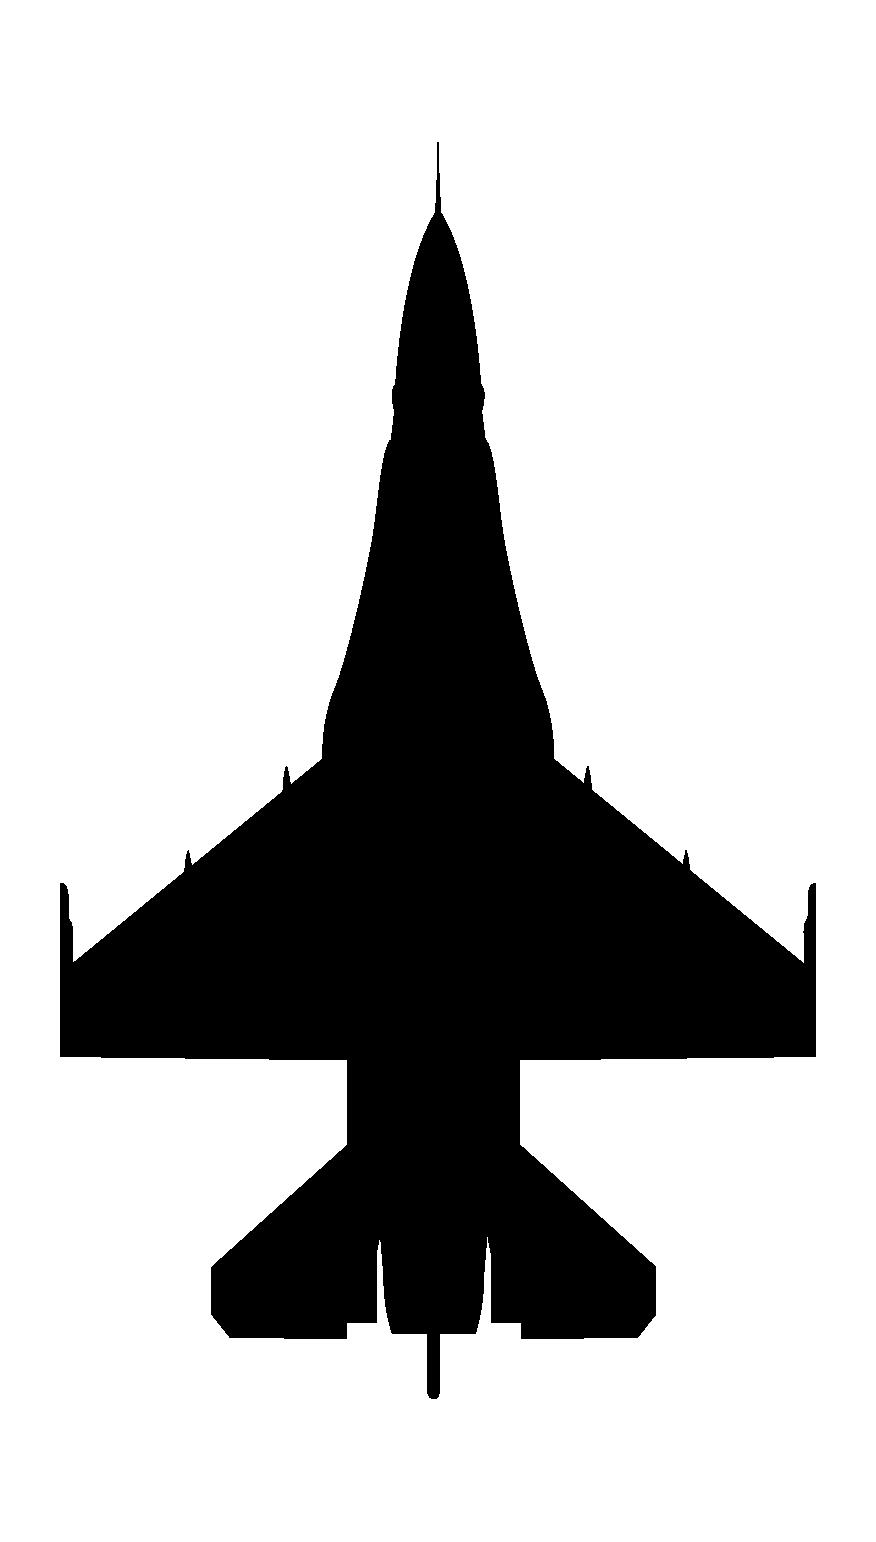
\includegraphics[
                        angle=180,
                        width=7.5mm,
                ]{diagrams/aircraft/silhouette_f16_top.pdf}};
            \draw[->, dashed]
                (mar)
                arc (180:90:5) 
                -- ++(5,0)
                arc (-90:0:5) 
                -- ++(0, 5)
                node[above, pos=1, ]{
                    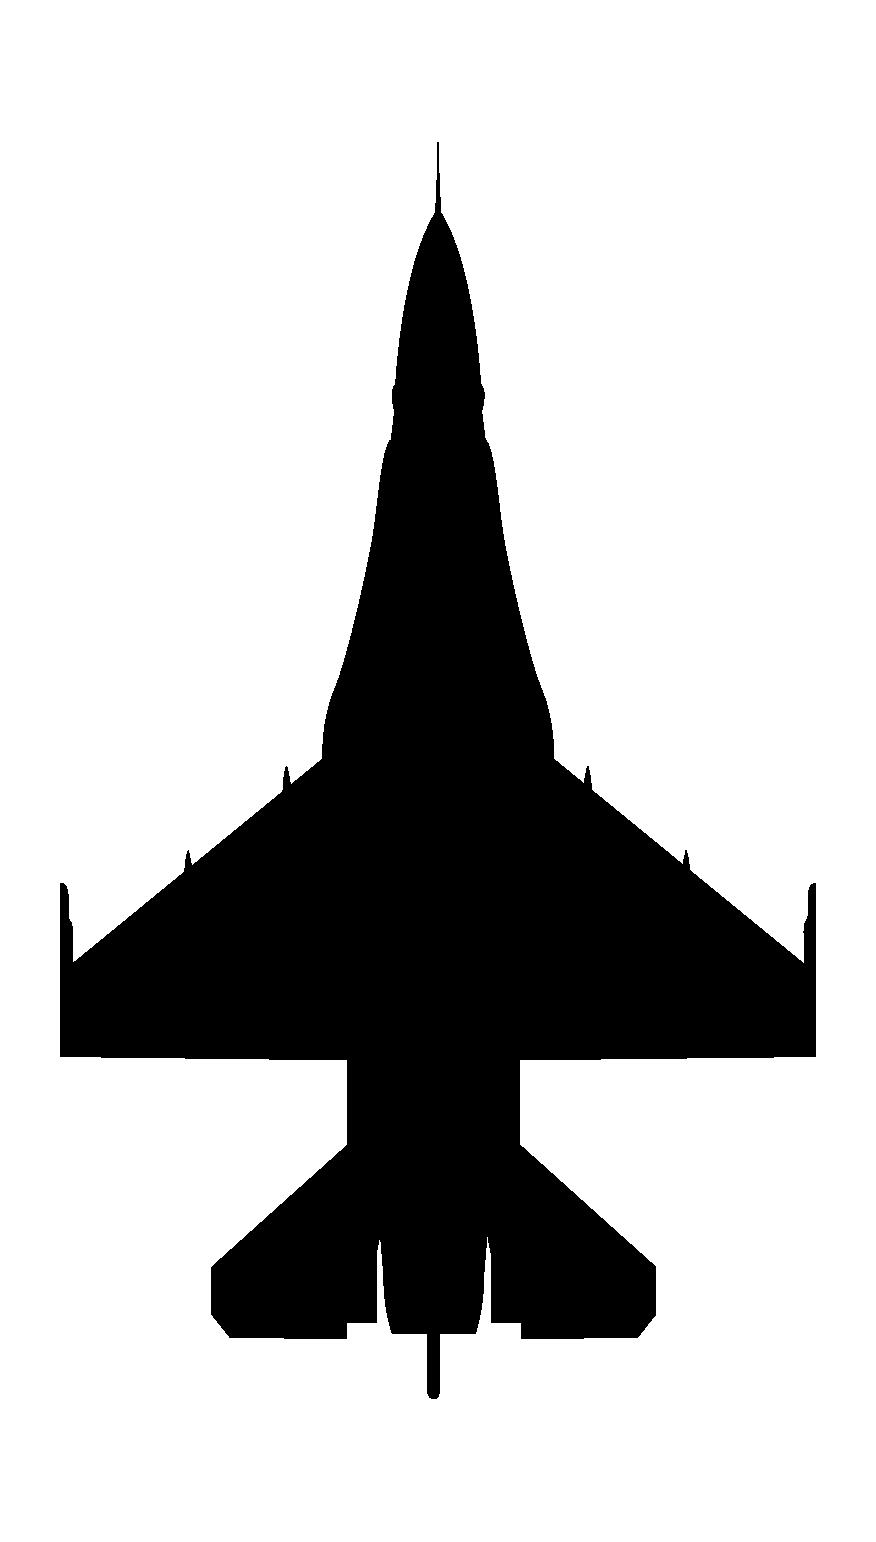
\includegraphics[
                        angle=0,
                        width=7.5mm,
                ]{diagrams/aircraft/silhouette_f16_top.pdf}};

            % bandit
            \node[] at (bandit) {
                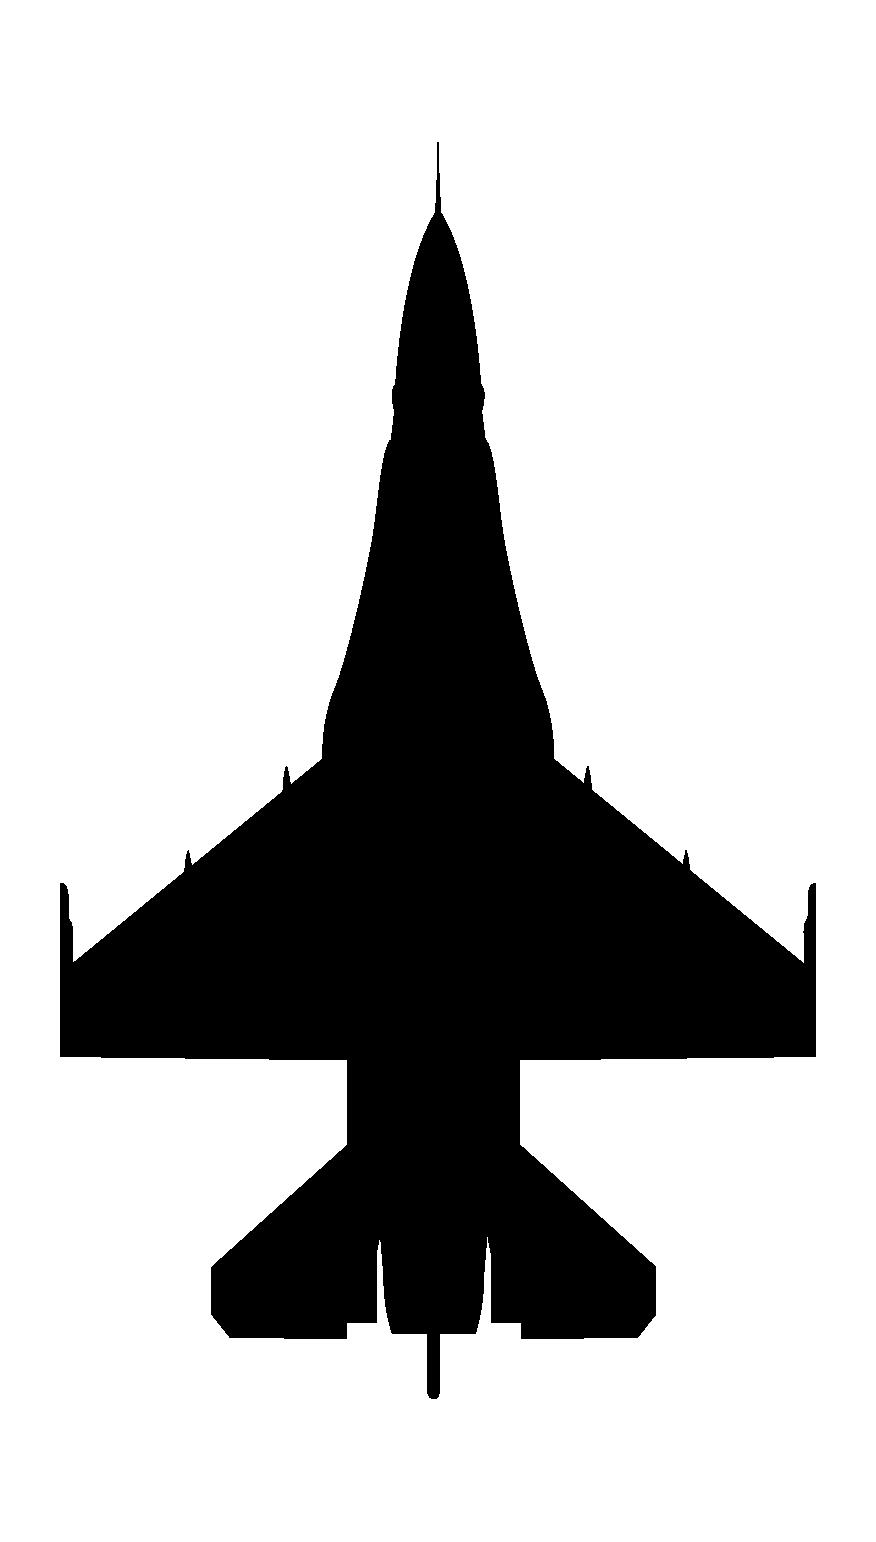
\includegraphics[
                    angle=180,
                    width=7.5mm,
            ]{diagrams/aircraft/silhouette_f16_top.pdf}};

            % labels
            \node[left, align=right, font=\small] at (cr) {
                \ref{subsec:ttpaa:timeline:shortskate:commit}
            };
            \node[left, align=right, font=\small] at (mtr) {
                \ref{subsec:ttpaa:timeline:shortskate:target}
            };
            \node[left, align=right, font=\small] at (sort) {
                \ref{subsec:ttpaa:timeline:shortskate:sort}
            };
            \node[left, align=right, font=\small] at (msr) {
                \ref{subsec:ttpaa:timeline:shortskate:shoot}
            };
            \node[left, align=right, font=\small] at (mar) {
                \ref{subsec:ttpaa:timeline:shortskate:abort}
            };

        \end{tikzpicture}
        \caption{Skate timeline}
        \label{fig:ttpaa:timeline:shortskate}
    }%
    \textbf{--- start of intercept timeline}
    \begin{itemize}
        \item AWACS picture or own FCR contacts meet briefed commit criteria
        \item flight leaves assigned patrol area
        \item \textbf{No later than CR}
    \end{itemize}

    \blueitem[Target]
    \label{subsec:ttpaa:timeline:shortskate:target}
    \begin{itemize}
        \item target call indicates responsibility to \\
        engage group in accordance with ROE
        \item flight members obtain radar contact
        \item \textbf{No later than MTR}
    \end{itemize}

    \blueitem[Sort]
    \label{subsec:ttpaa:timeline:shortskate:sort}
    \begin{itemize}
        \item flight members sort contacts
        \item flight members obtain FCR lock on assigned contact
    \end{itemize}

    \blueitem[MRM Employment]
    \label{subsec:ttpaa:timeline:shortskate:shoot}
    \begin{itemize} 
        \item verify clear avenue of fire
        \item \textbf{DLZ} --- R\textsubscript{TR} to R\textsubscript{PI} 
        \hfill (see \cref{fig:ttpaa:timeline:shortskate:dlz})\\
        manual loft to maximize performance
        \item \textbf{crank post launch to minimize closure}
        \item \textbf{within TR to increase P\textsubscript{K}}
        \item \textbf{No later than MSR}
        \item \textbf{no option to recommit and engage before MAR}
    \end{itemize}
    
    \marginpar{
        \captionsetup{type=figure}
        \centering
        \begin{tikzpicture}[figstyle]
            \node[boxedmarfigstyle] (fig) at (0,0) {
                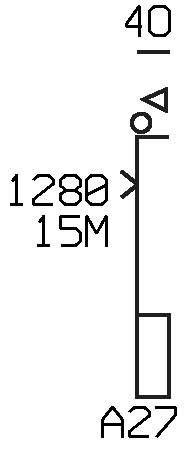
\includegraphics[
                    scale=0.5,
                ]{mfd/fcr_aa/aim120_subfig_dlz_prelaunch.pdf}
            };
        \end{tikzpicture}
        \caption{DLZ for short skate}
        \label{fig:ttpaa:timeline:shortskate:dlz}
    }
    \blueitem[Abort]%
    \label{subsec:ttpaa:timeline:shortskate:abort}
    \textbf{--- 5G slicing turn at MAR}
\end{checklistenumerate}

\marginfigrestore